\documentclass{standalone}
\usepackage{hsbcommon}
\begin{document}
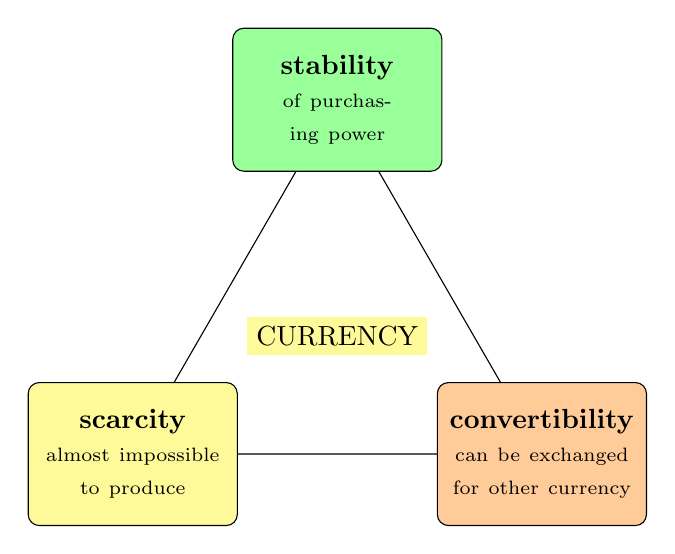
\begin{tikzpicture}[rotate=-30]
    \def\diamond{3}
    \node[fill=yellow!40] (M) at (0:0) {CURRENCY};
    \draw (0:\diamond) -- (120:\diamond) -- (240:\diamond)  -- cycle;
    \foreach [count=\i] \myfunc/\myexpl/\mycol in {
        stability/of purchasing power/green,
        scarcity/almost impossible to produce/yellow,
        convertibility/can be exchanged for other currency/orange%
    }
    {
        \node[draw,rounded corners,fill=\mycol!40,text width=16ex,minimum height=12ex,align=center] (\i) at (\i*120:\diamond) {
            \textbf{\myfunc}\\ {\scriptsize\myexpl}
        };
    }
    % \node[draw=none] (time) [rotate=45,inner sep=-1.5ex,ellipse,thick,fit={(3) (4)}] {};
    %  % \ifstep{1,time}{
    %     \begin{scope}[red]        
    %         \node(time) [draw, rotate=45,inner sep=-1.5ex,ellipse,thick,fit={(3) (4)}] {};
    %         \node[fill=white] at (time) {in time};
    %     \end{scope}
    %  % }
    
\end{tikzpicture}
\end{document}